\documentclass{article}
\usepackage[a4paper, margin=1in]{geometry}
\usepackage{graphicx} % Required for inserting images
\usepackage{amsmath}
\usepackage[style=numeric, backend=biber]{biblatex}
\addbibresource{References.bib}

\title{Students' Grade Performance Based on Lifestyle and Health Factors}
%\author{Guilherme Cruz & João Piedade}
%\date{September 2024}


\begin{document}
\maketitle

\section{Introduction}
\quad Machine learning has consistently demonstrated its utility and power in addressing real-world problems across a wide range of fields. When it comes to evaluating performance, particularly academic grade performance, numerous variables must be taken into account.

In this study, we will train our machine learning (ML) models using a dataset obtained from Kaggle. These models will aid both students and educators in understanding which factors most significantly influence students' grades.

Our report will begin with a Problem Formulation section, where we will clearly define the problem and outline how we intend to leverage ML models to address it. Following this, a Methods section will provide a detailed analysis of the models considered and their evaluation based on criteria such as accuracy.

In the Results section, we will present the outcomes derived from our models, followed by an in-depth analysis. Finally, the key findings will be synthesized and summarized in the Conclusion section.

\section{Problem Formulation}
\quad Our problem consists on understand how student's lifestyle and health factors affect their academic performance, so will use supervised learning models.
This study examines this problem and will try to answer and to come up with a connection between the student's lifestyle and health factors with their academic performances. We used a dataset from Kaggle \cite{Kaggle_dataset} that includes a combination of categorical and continuous variables, which influenced our choice of machine learning models.


Each datapoint represents a student and includes features related to their lifestyle. These features consist of Hours Studied, Class Attendance, Access to Resources, Previous Test Scores, Parental Involvement, and Extracurricular Activities. For our analysis, we chose to focus on features that relate more closely to lifestyle and health, specifically Parental Involvement, Extracurricular Activities, Sleep Hours, Physical Activity, and Peer Influence.

The label we selected is the Exam Score, as it provides a clear measure of academic performance. By exploring the connections between these lifestyle factors and exam scores, we hope to uncover insights into how they impact students’ educational outcomes.

\section{Methods}

\quad As our dataset contained both continuous and categorical values, the selection of machine learning (ML) methods was mainly influenced by this characteristic. With 6,607 datapoints and originally 20 columns, we decided to focus on only five key features for our problem. These features were chosen based on their direct relevance to students' health and lifestyle, which we believe they have significantly impact on the academic performance. The selected features include parental involvement, extracurricular activities, sleep hours, physical activity, and peer influence. The label for our analysis was straightforward, as it was the only one that works in our problem: the student exam scores, being a good indicator of academic performance.

The reason behind for choosing these specific features lies in their established correlation with academic outcomes. For instance, parental involvement is often linked to higher student motivation and engagement, while adequate sleep and physical activity are critical for cognitive function and overall well-being. By having a less number of features, getting rid of the ones that weren’t crutial for our problem, we aimed to avoid the overfitting. 

We were between using K-Fold Cross Validation (K-Fold) or splitting the dataset in two parts (training set and test set). As our dataset is quite large, we concluded that the best approach  would be to use K-Fold with 10 splits. We implemented this technique as it would provide more reliable and robust estimates of the model performance compared to a simple train-test split. This approach allow us to evaluate how well the model generalizes across different subsets of the data reducing the risk of overfitting. \cite{K-fold_Cross-Validation}

As we had both categorical and continuous values, we knew that our ML model choice would have to be between models that could be trained with either types of values together such as Decision Tress, Random Forest, Support Vector Classification, etc. Due to the presence of both types of values, we had to implement the LabelEnconder function from the sklearn preprocessing module, which was used to convert categorical variables into numerical format, enabling their integration in models mentioned earlier.\cite{ML_Model}

In order to choose between Random Forest Model or Decision Tress and Support Vector Classification, we decided to do some tests and carefully analyse how they differ from each other to see witch model would better suit our interests.

\subsection{Random Forest and Decision Trees}

\quad The reason why we combine Random Forest and Decision trees models in the same subsection is easy. Basically, the Random Forest model is a combination of many decision trees. So we will now analyse the decision trees model. 

A decision tree is a supervised learning algorithm that starts with a single node (denominated by root) and splits into branches based on decisions made on each nodes. Basically, at each node the algorithm chooses a feature and a threshold value to split the data. \cite{Randon_Forest} On our case, it might split based on whether a student's study hours are above or below a certain number. This methods is recursively and at the end, the final nodes represent the outcome. They are easy to understand and we can follow the decisions made to get to the conclusion, however we can easily have overfitting problems, which means that we would have a great accuracy for our trained data, but a really poor one on our validation set. \cite{Random_Forest_Library}

To mitigate this problem, Random Forest is often used since it predicts more accurate results, particularly when the individual trees are uncorrelated with each other.

\subsection{Support Vector Classification - SVC}

\quad Support Vector Classification is a specialized form of the Support Vector Machine, designed specifically for classification tasks. The model works by distinguishing between two classes through the identification of an optimal hyperplane that maximizes the margin between the closest data points from opposing classes. \cite{SVM}

SVM is valuable due to its ability to manage non-linear relationships using the kernel trick, which reconfigured input data into a higher-dimensional space where linear separation becomes possible. In essence, the algorithm searches for the best hyperplane to separate the two classes while maximizing the margin. Once the support vectors—the points closest to the hyperplane—are identified, the model calculates the hyperplane by maximizing the distance between it and the support vectors. After establishing the hyperplane, new data points are classified based on which side of the boundary they fall.

A major strength of this model is its versatility. The kernel trick allows it to handle non-linear decision boundaries, making it particularly effective when the number of features exceeds the number of data points. However, SVM's performance tends to decline as dataset size increases, and selecting the right kernel and tuning parameters (C and gamma) can be difficult, often requiring cross-validation for optimization.

\subsection{ML Model Decision}

In this section, we evaluate the performance of the machine learning models employed in our analysis, specifically focusing on Random Forest and Support Vector Classification (SVC). The training accuracy for the Random Forest model was 91.91\%, while the SVC achieved a slightly higher training accuracy of 94.49\%. Similarly, during validation, the Random Forest model produced an accuracy of 90.87\%, compared to 94.41\% for SVC. 

The results indicate that while both models performed well, SVC exhibited superior accuracy in both training and validation phases. This suggests that SVC may be better suited for the dataset at hand, particularly in distinguishing between the classes with a more nuanced decision boundary.

A key factor in the performance of SVC is the hinge loss function, which plays a crucial role in optimizing the model. Hinge loss is used primarily in SVM models and is defined as follows\cite{Hinge-loss}:

\[
\text{Hinge Loss} = \max(0, 1 - y_i \cdot f(x_i))
\]


In this equation, \(y_i\) represents the true label of the data point, and \(f(x_i)\) is the output of the model for that data point. The hinge loss penalizes misclassifications and encourages correct classifications to be made with a margin. Specifically, the loss is zero when the prediction is correct and lies beyond the margin (i.e., \(y_i \cdot f(x_i) > 1\)). However, as soon as a prediction falls within the margin or is incorrect, the loss increases, leading to adjustments in the model.\cite{Predicting_Wine_Quality}

The use of hinge loss allows SVC to focus not just on correctly classifying points but also on maximizing the margin, ultimately contributing to the model’s robustness. Given the results of our model comparison (Fig \ref{fig:enter-label}), it appears that SVC's ability to effectively utilize hinge loss, alongside the kernel trick for managing non-linear relationships, provides a significant advantage over Random Forest in this context.


\begin{figure}
    \centering
    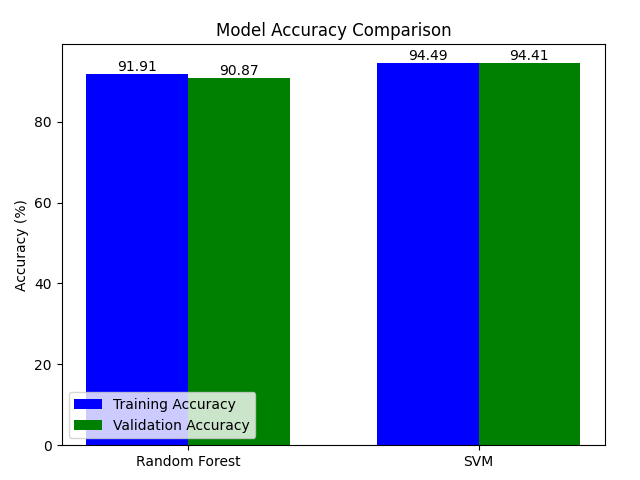
\includegraphics[width=0.5\linewidth]{Figure_1.png}
    \caption{Model Accuracy Comparison}
    \label{fig:enter-label}
\end{figure}


\printbibliography

\section{Appendix}

The link for the repository: \url{https://github.com/guilhermecruz760/Aalto-Machine-Learning-Project}

\end{document}
